\section{eo\-Bit$<$ Fit\-T $>$ Class Template Reference}
\label{classeo_bit}\index{eoBit@{eoBit}}
Implementation of bitstring chromosome.  


{\tt \#include $<$ga/eo\-Bit.h$>$}

Inheritance diagram for eo\-Bit$<$ Fit\-T $>$::\begin{figure}[H]
\begin{center}
\leavevmode
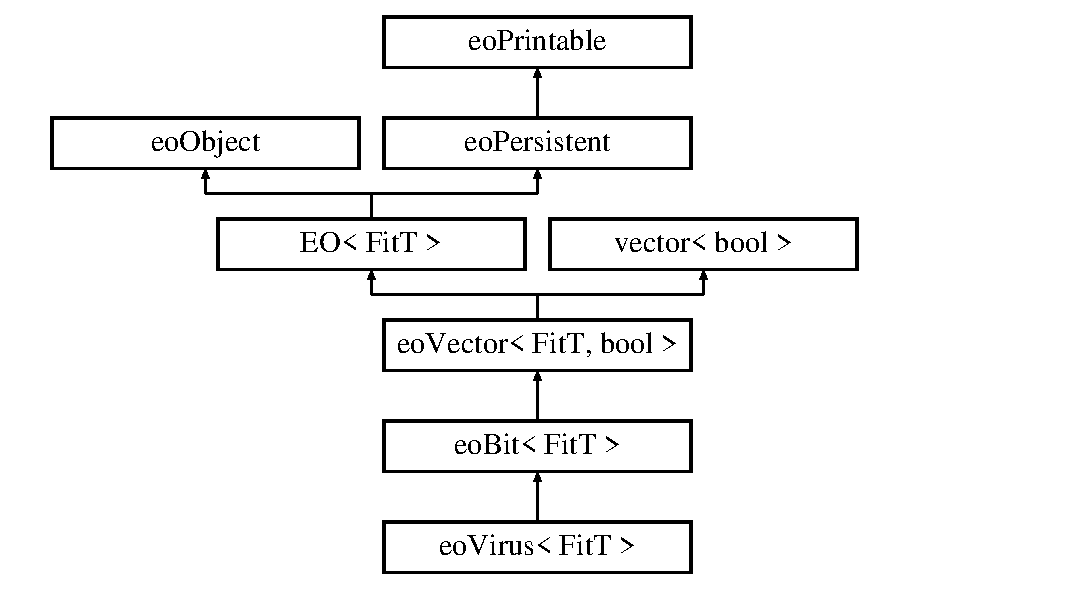
\includegraphics[height=6cm]{classeo_bit}
\end{center}
\end{figure}
\subsection*{Public Member Functions}
\begin{CompactItemize}
\item 
{\bf eo\-Bit} (unsigned size=0, bool value=false)
\begin{CompactList}\small\item\em (Default) Constructor. \item\end{CompactList}\item 
virtual std::string {\bf class\-Name} () const \label{classeo_bit_a1}

\begin{CompactList}\small\item\em My class name. \item\end{CompactList}\item 
virtual void {\bf print\-On} (std::ostream \&os) const 
\begin{CompactList}\small\item\em To print me on a stream. \item\end{CompactList}\item 
virtual void {\bf read\-From} (std::istream \&is)
\begin{CompactList}\small\item\em To read me from a stream. \item\end{CompactList}\end{CompactItemize}


\subsection{Detailed Description}
\subsubsection*{template$<$class Fit\-T$>$ class eo\-Bit$<$ Fit\-T $>$}

Implementation of bitstring chromosome. 

Based on STL's vector$<$bool$>$ specialization. 



Definition at line 56 of file eo\-Bit.h.

\subsection{Constructor \& Destructor Documentation}
\index{eoBit@{eo\-Bit}!eoBit@{eoBit}}
\index{eoBit@{eoBit}!eoBit@{eo\-Bit}}
\subsubsection{\setlength{\rightskip}{0pt plus 5cm}template$<$class Fit\-T$>$ {\bf eo\-Bit}$<$ {\bf Fit\-T} $>$::{\bf eo\-Bit} (unsigned {\em size} = {\tt 0}, bool {\em value} = {\tt false})\hspace{0.3cm}{\tt  [inline]}}\label{classeo_bit_a0}


(Default) Constructor. 

\begin{Desc}
\item[Parameters:]
\begin{description}
\item[{\em size}]Size of the binary std::string. \end{description}
\end{Desc}


Definition at line 69 of file eo\-Bit.h.

\subsection{Member Function Documentation}
\index{eoBit@{eo\-Bit}!printOn@{printOn}}
\index{printOn@{printOn}!eoBit@{eo\-Bit}}
\subsubsection{\setlength{\rightskip}{0pt plus 5cm}template$<$class Fit\-T$>$ virtual void {\bf eo\-Bit}$<$ {\bf Fit\-T} $>$::print\-On (std::ostream \& {\em os}) const\hspace{0.3cm}{\tt  [inline, virtual]}}\label{classeo_bit_a2}


To print me on a stream. 

\begin{Desc}
\item[Parameters:]
\begin{description}
\item[{\em os}]The std::ostream. \end{description}
\end{Desc}


Reimplemented from {\bf eo\-Vector$<$ Fit\-T, bool $>$} {\rm (p.\,\pageref{classeo_vector_a4})}.

Definition at line 82 of file eo\-Bit.h.

References EO$<$ F $>$::print\-On().\index{eoBit@{eo\-Bit}!readFrom@{readFrom}}
\index{readFrom@{readFrom}!eoBit@{eo\-Bit}}
\subsubsection{\setlength{\rightskip}{0pt plus 5cm}template$<$class Fit\-T$>$ virtual void {\bf eo\-Bit}$<$ {\bf Fit\-T} $>$::read\-From (std::istream \& {\em is})\hspace{0.3cm}{\tt  [inline, virtual]}}\label{classeo_bit_a3}


To read me from a stream. 

\begin{Desc}
\item[Parameters:]
\begin{description}
\item[{\em is}]The std::istream. \end{description}
\end{Desc}


Reimplemented from {\bf eo\-Vector$<$ Fit\-T, bool $>$} {\rm (p.\,\pageref{classeo_vector_a5})}.

Definition at line 94 of file eo\-Bit.h.

References EO$<$ F $>$::read\-From().

The documentation for this class was generated from the following file:\begin{CompactItemize}
\item 
eo\-Bit.h\end{CompactItemize}
